\section{Introduction}\label{introduction}

An \emph{interactive indoor mapping} environment consists of a virtual reconstruction
of a physical indoor space, in which the user can move around and interact
with virtual objects, that are found in the same position they actually occupy in the
real world. Such an interactive indoor mapping can be thought as a specialized
and very evoluted \emph{user interface} capable of giving a glimpse of a section of
the real world that the user can handle in a natural and intuitive way.  Such
a reconstructed virtual indoor environment can be considered a general
platform where many different applications can rely upon. Both promising and
already well explored ICT applications may find in \emph{virtual indoor mapping} the
perfect context to be integrated into.

In particular, for environments with massive presence of sensor-equipped (or
``smart'') objects, which realize the so-called \emph{IoT} (Internet of
Things), the interactive indoor mapping represents an ideal integrated
interface for IoT monitoring systems. To be specific, it can be the container
of indoor navigation systems, giving the user, to be routed across an indoor
environment, the opportunity to interact with objects along the suggested
paths. Futhermore, in conjunction with the advancements in the field of user
indoor location, whose efforts are nowdays focused to realize an integration
of positioning systems like GNSS (Global Navigation Satellite system), Wi-Fi, Bluetooth and 
LTE (Long Term Evolution), to support continuos outdoor/indoor navigation by
means of integration tecnology like for example SDR (Software Defined Radio),
it represents the most natural interface to perform realtime access monitoring
and multiperson tracking.

To enable such a interactive mapping platform it is of the utmost importance to set up  a
descriptive representation of the indoor environment. This description belongs to 
the field of indoor cartography, which as digital evolution of plain floor
plans, has arrived to arouse the interest of big players like Google, that has
integrated indoor plans of specific locations of interest
\cite{indoormaps}  into Google Maps. In general, can be considered ``of interest'' --- such to
justify and motivate indoor cartographic applications --- both public or
commercial places of vast dimensions, as for example airports, train stations,
shopping malls, and also private buildings subject to strict access protocols,
like warehouses, logistics centers, datacenters, etc.

Despite of the growing attention regarding indoor cartography, efforts to specify
open formats for indoor representation are few and partial, and certainly not
intended to support the interactive indoor mapping, which is conversely the
main purpose of this paper.

This work, jointly developed by Sogei S.p.A., an ICT company fully owned by
Italian  Ministry of Economy and Finance, and the CVDLAB (Computational Visual
Design Laboratory) of the ``Roma Tre'' University, is inspired by the
necessities of Sogei itself, which runs one of the largest data center in
Europe, so requiring strict access control policies, which include the
recording and  the real-time interaction with man/machine maintenance
scenarios. Support for tis interactive framework, where real-time awarness of
the maintainer position inside the data center helps to reduce intervention
times and to increase safety and security, has been chosen as case study of
interactive indoor mapping, based on the proposed indoor cartographic format.


The remainder of this document is organized as follows. In
Section~\ref{related-work} we provide an overview of the state of the art in
the field of indoor document standards and related applications.
Section~\ref{advances} is devoted to describe the advances introduced by the
novel cartographic document proposed, while section~\ref{hijson-syntax}
presents the document syntax. Section~\ref{hijson-toolkit} reports about the
toolkit specifically developed to handle the new document format. In
Section~\ref{hjson-web-framework} it is depicted the overall architecture and
the implementation of the web based application framework, which is in turn
used to achieve the objectives stated above. Section~\ref{case-study} presents
a case-study application of the document format discussed in this paper.
Finally, Section~\ref{conclusions} proposes some conclusive remarks and future
developments.


\begin{figure*}[!htbp] % figure placement: here, top, bottom, or page
 \centering
 % 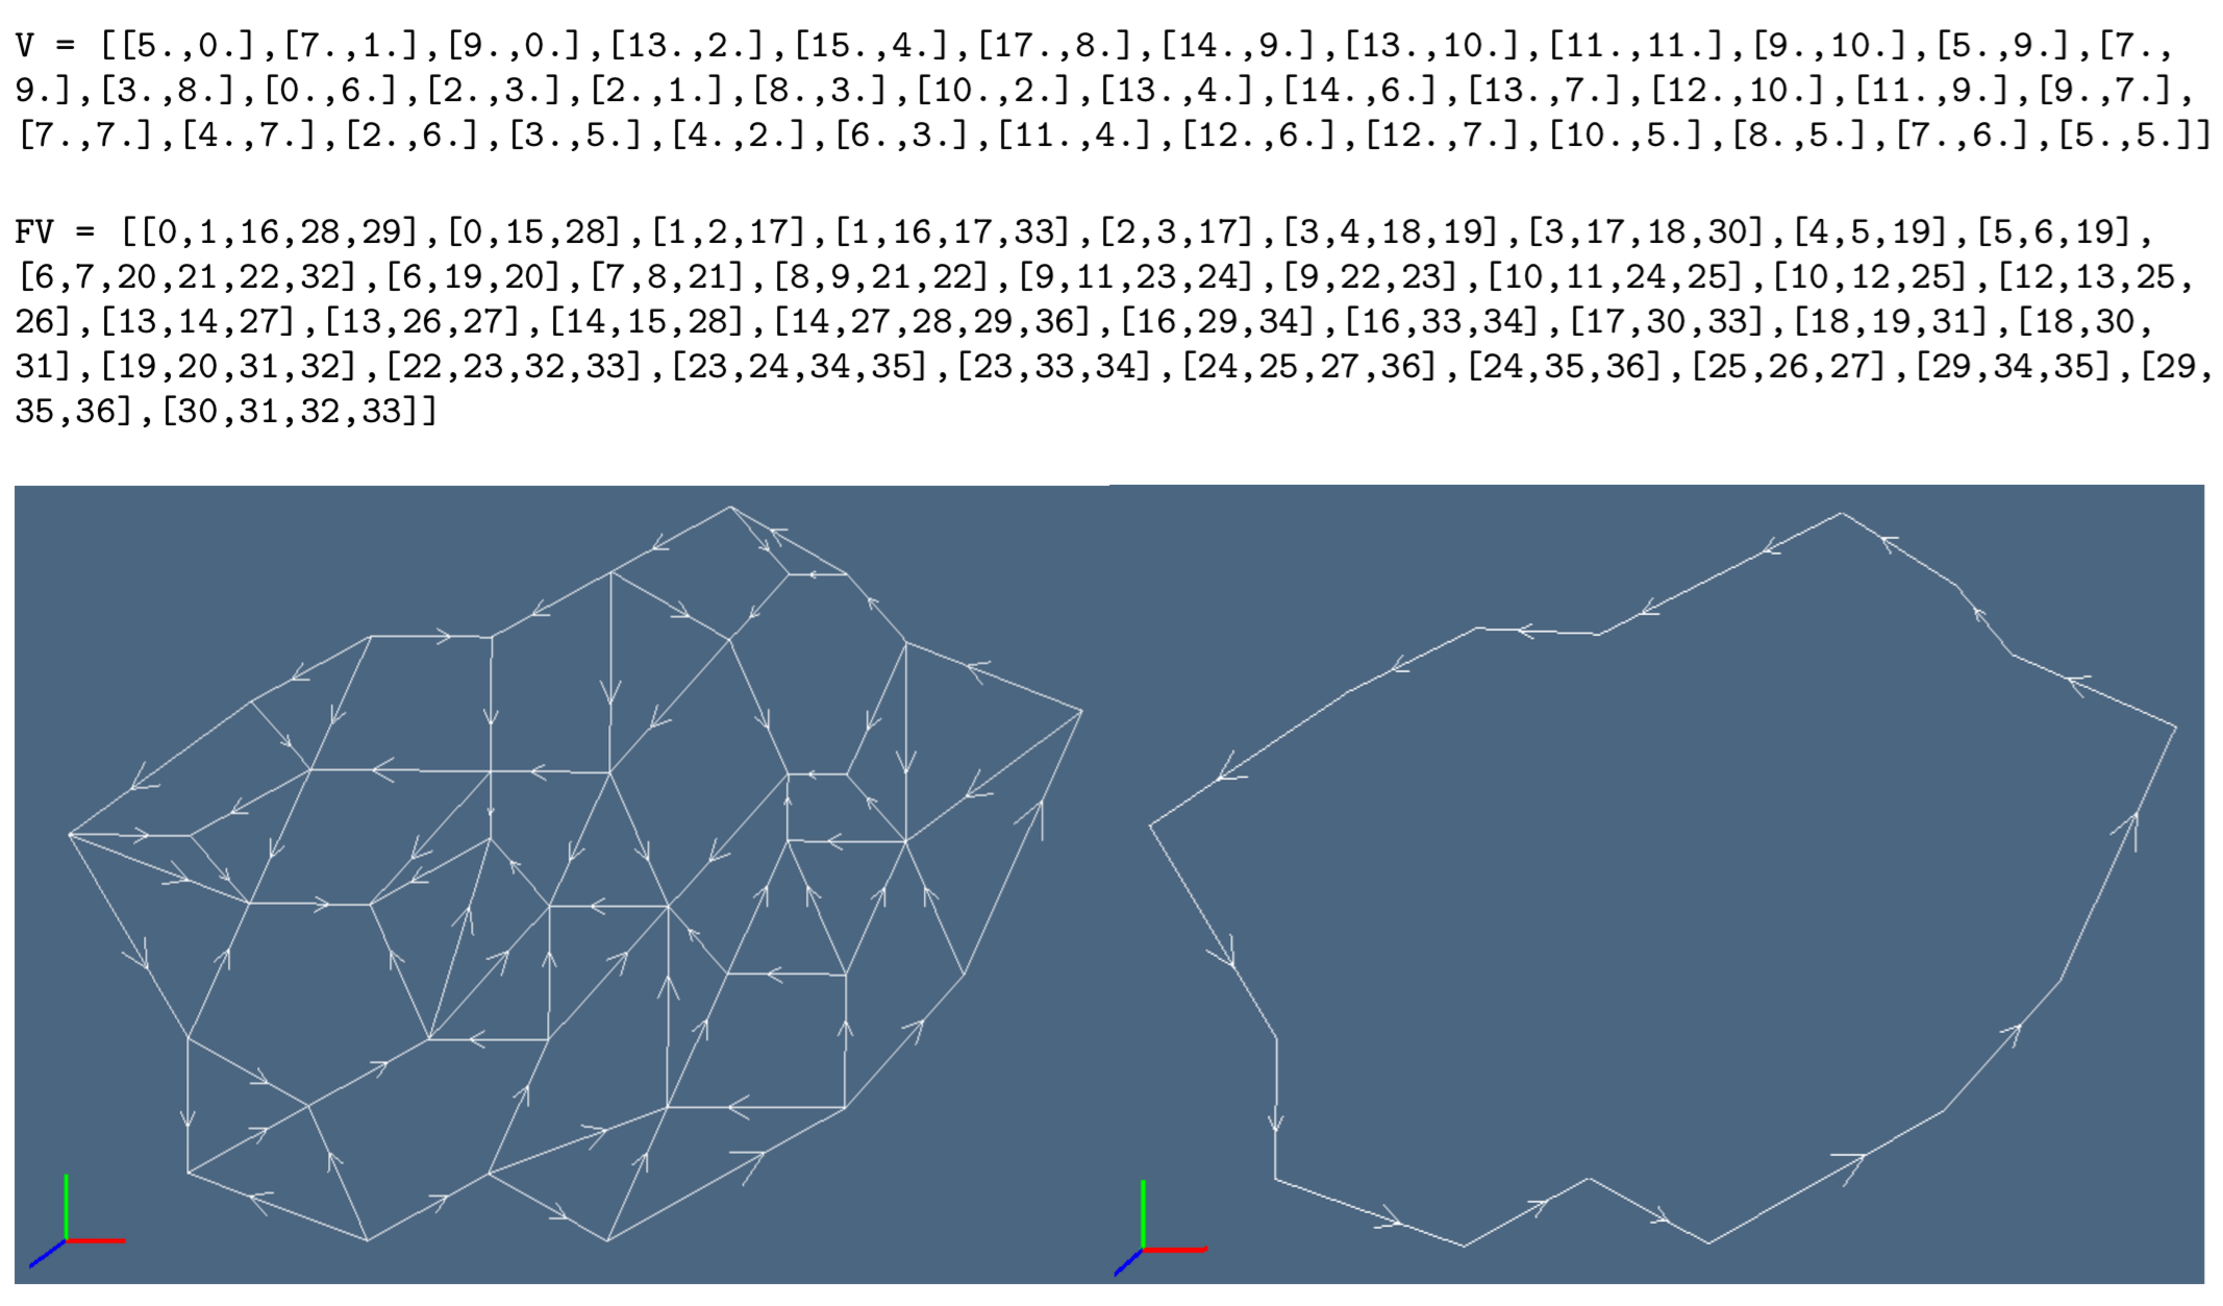
\includegraphics[width=0.5\linewidth]{images/minimum} 
 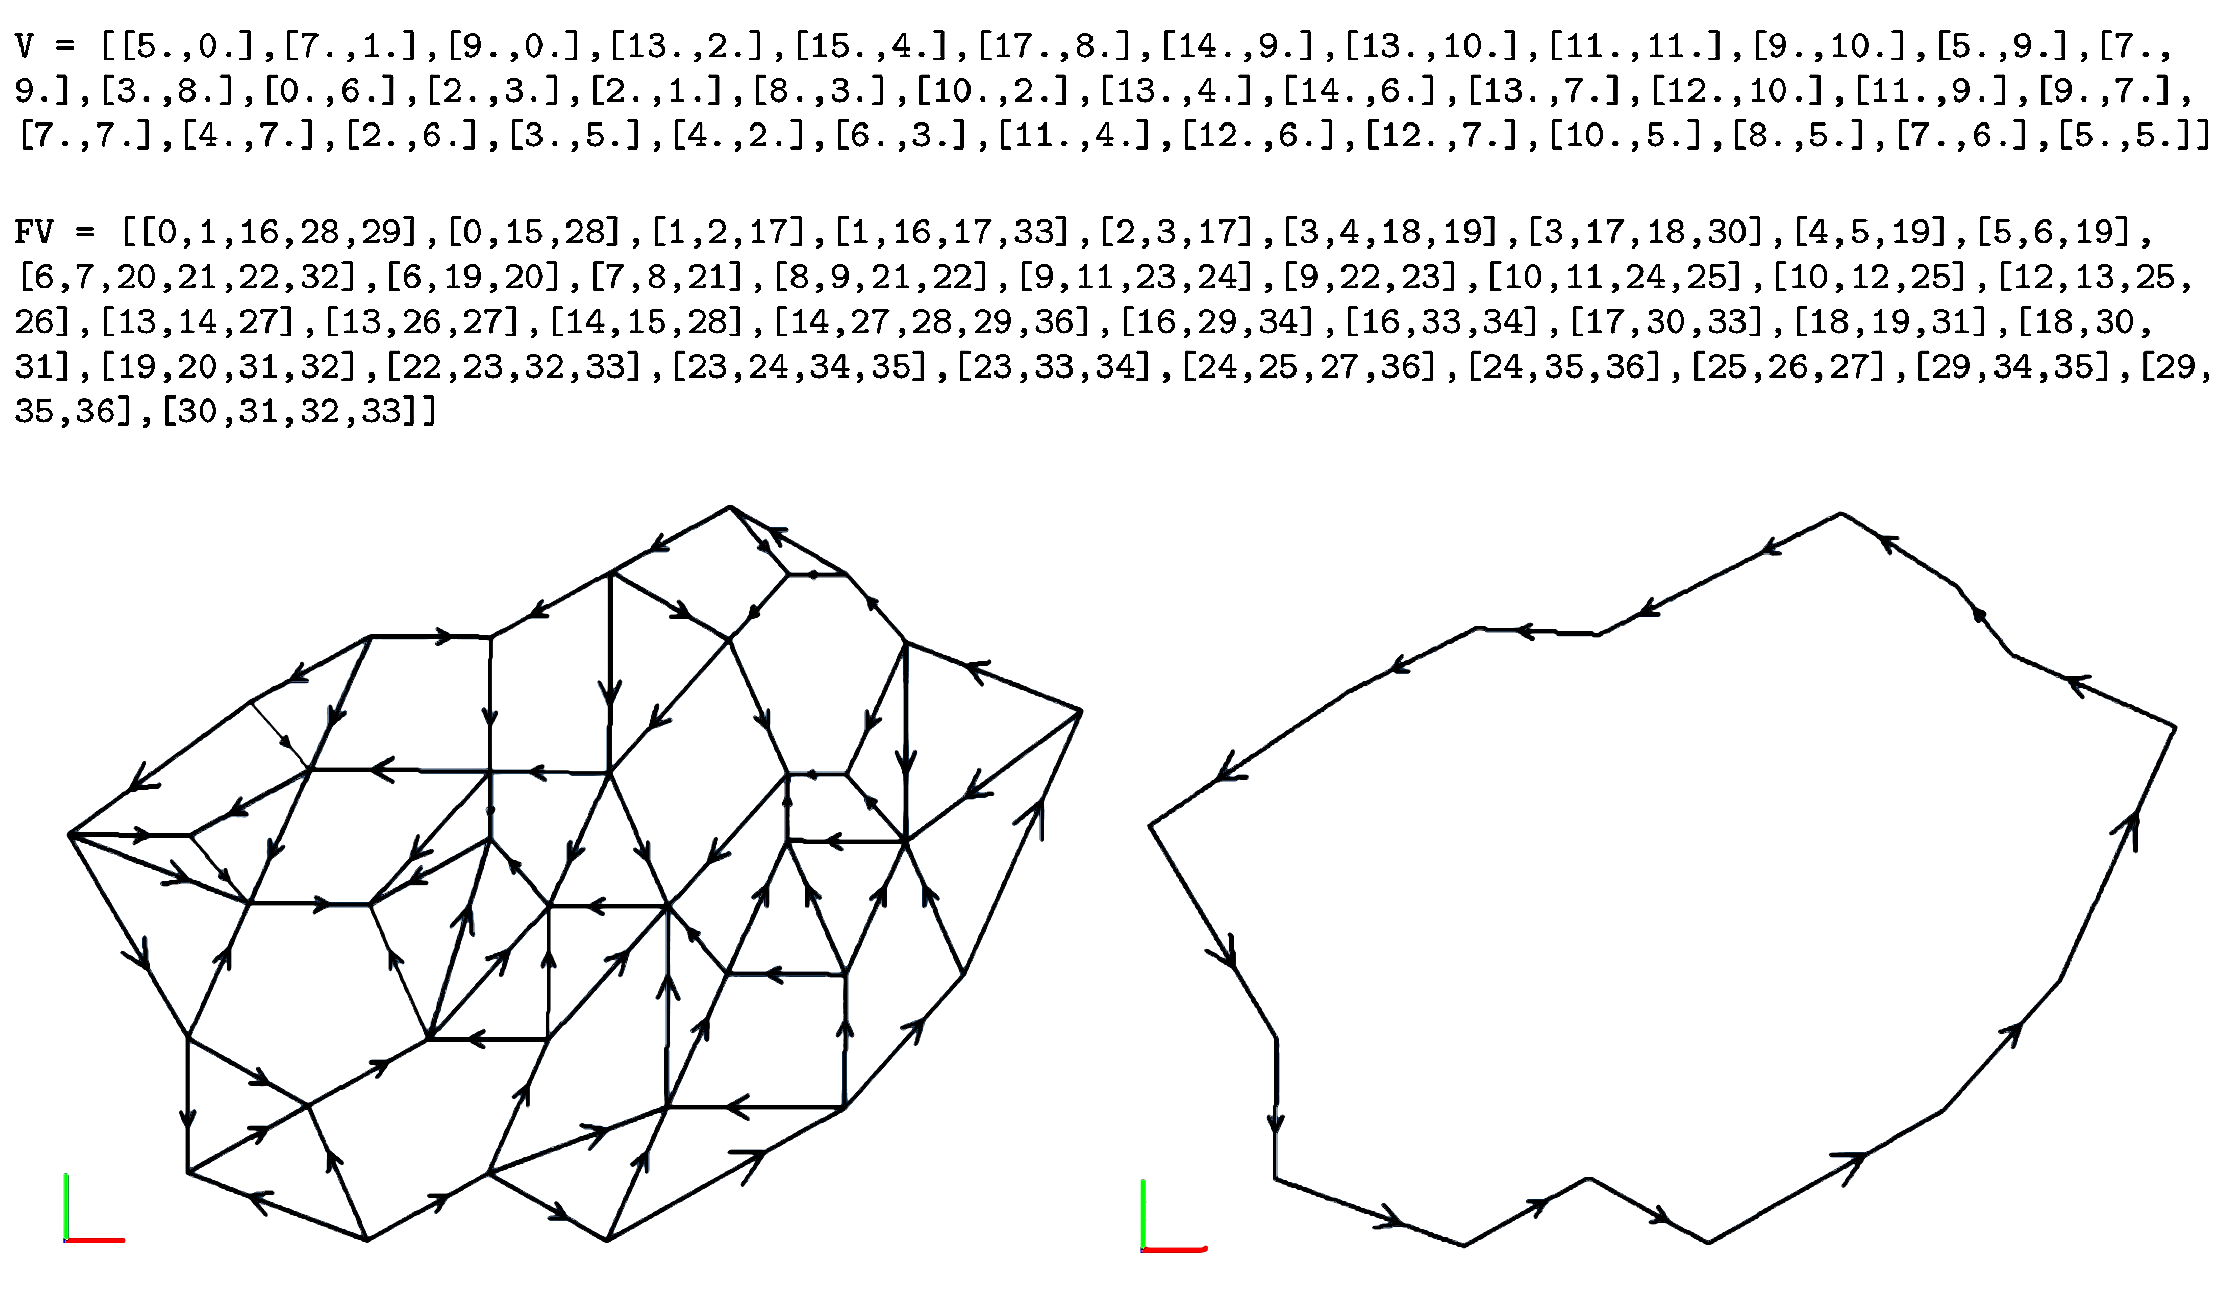
\includegraphics[width=0.5\linewidth]{images/minimum-colors-test} 
 \hfill
 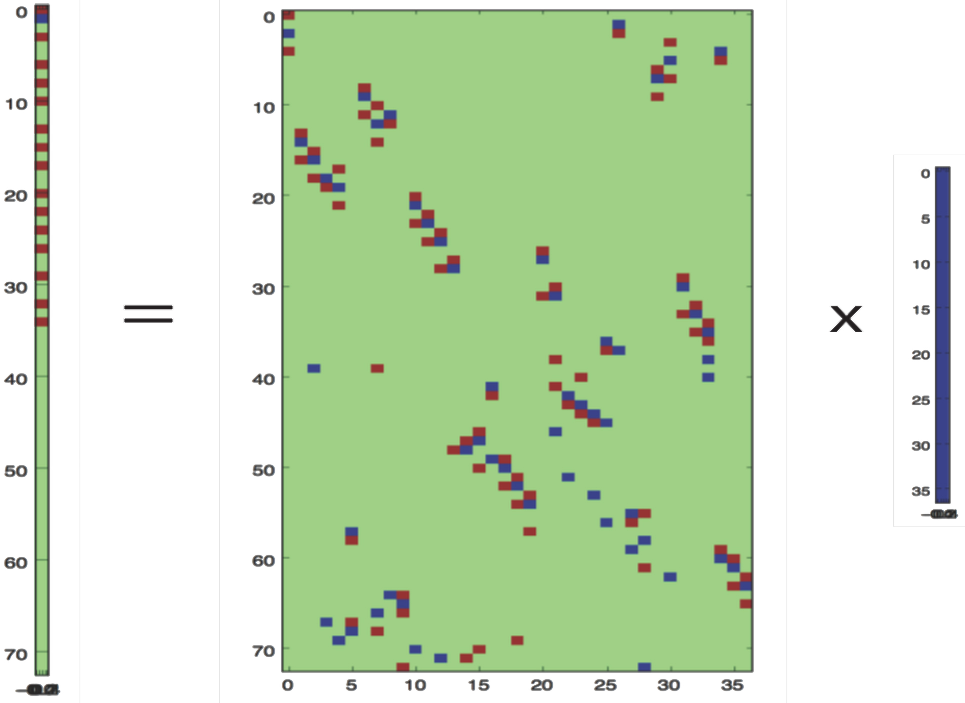
\includegraphics[width=0.4\linewidth]{images/boundary} 
 \caption{A toy example of the LAR scheme: (a) the bare minimum of data with \emph{complete} information about topology; (b) the extracted boundary; (c) the extraction method $[e] = [\partial][f]$ giving the coordinate representation (in the discrete basis of the 1-cells) of the boundary edges $[e]$ by product of the sparse boundary operator matrix $[\partial]$ times the coordinate representation $[f]$ of the 2-cells (faces), in the discrete basis of the 2-cells.}
 \label{fig:minimum}
\end{figure*}


% \begin{figure}[!h]
%  \centering
%  \begin{subfigure}[b]{\linewidth}
%  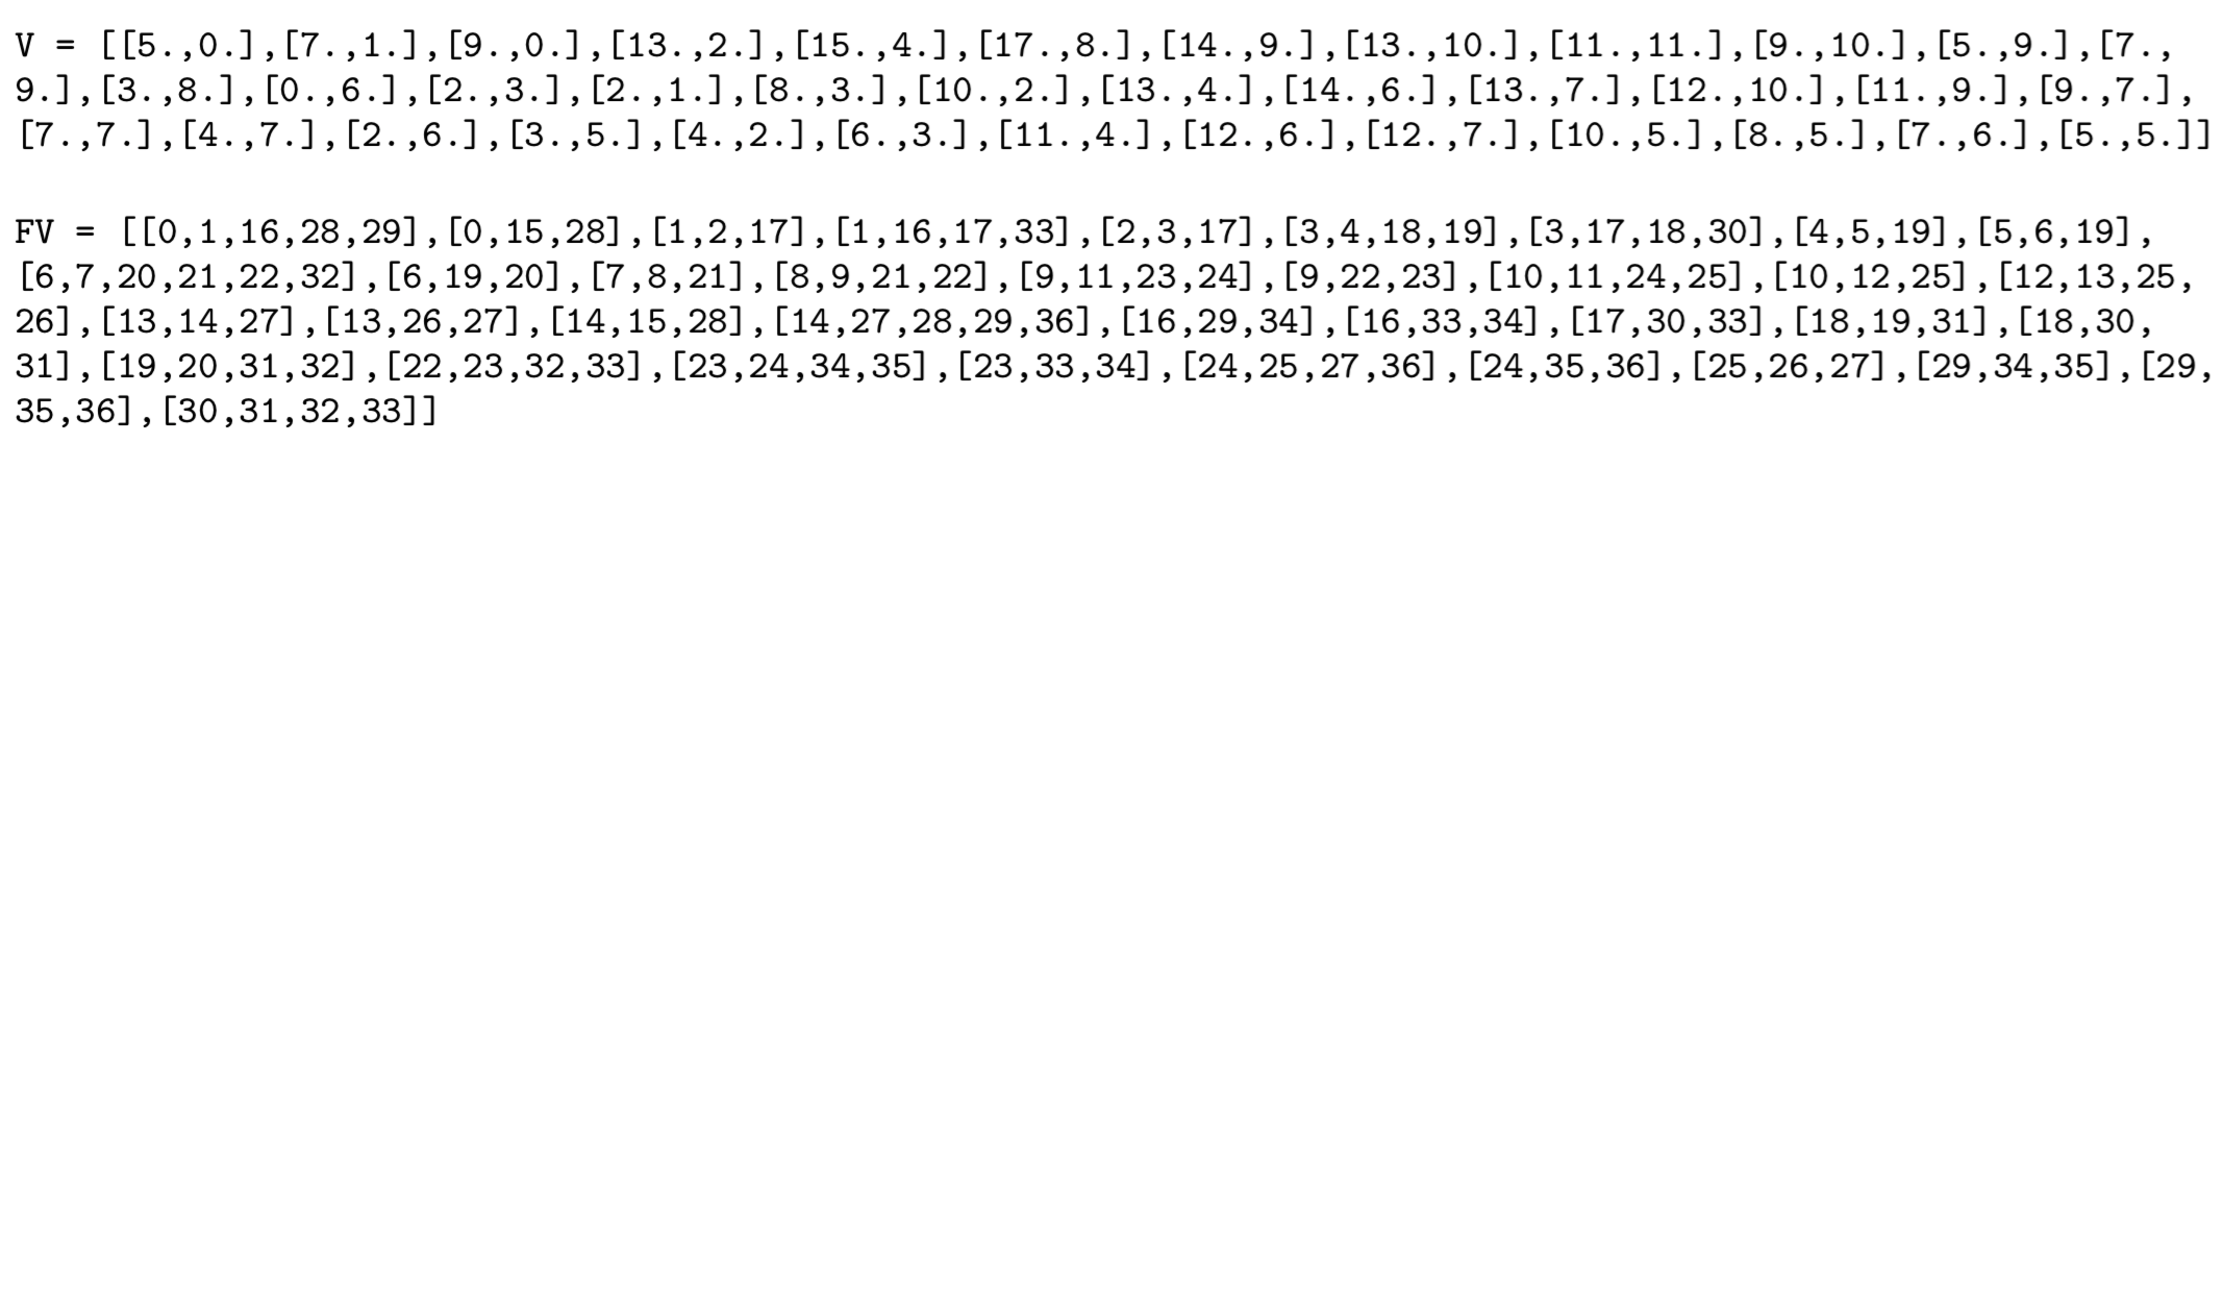
\includegraphics[width=\textwidth]{images/minimum-data}
%  \end{subfigure}
% \\
%  \begin{subfigure}[b]{0.48\linewidth}
%  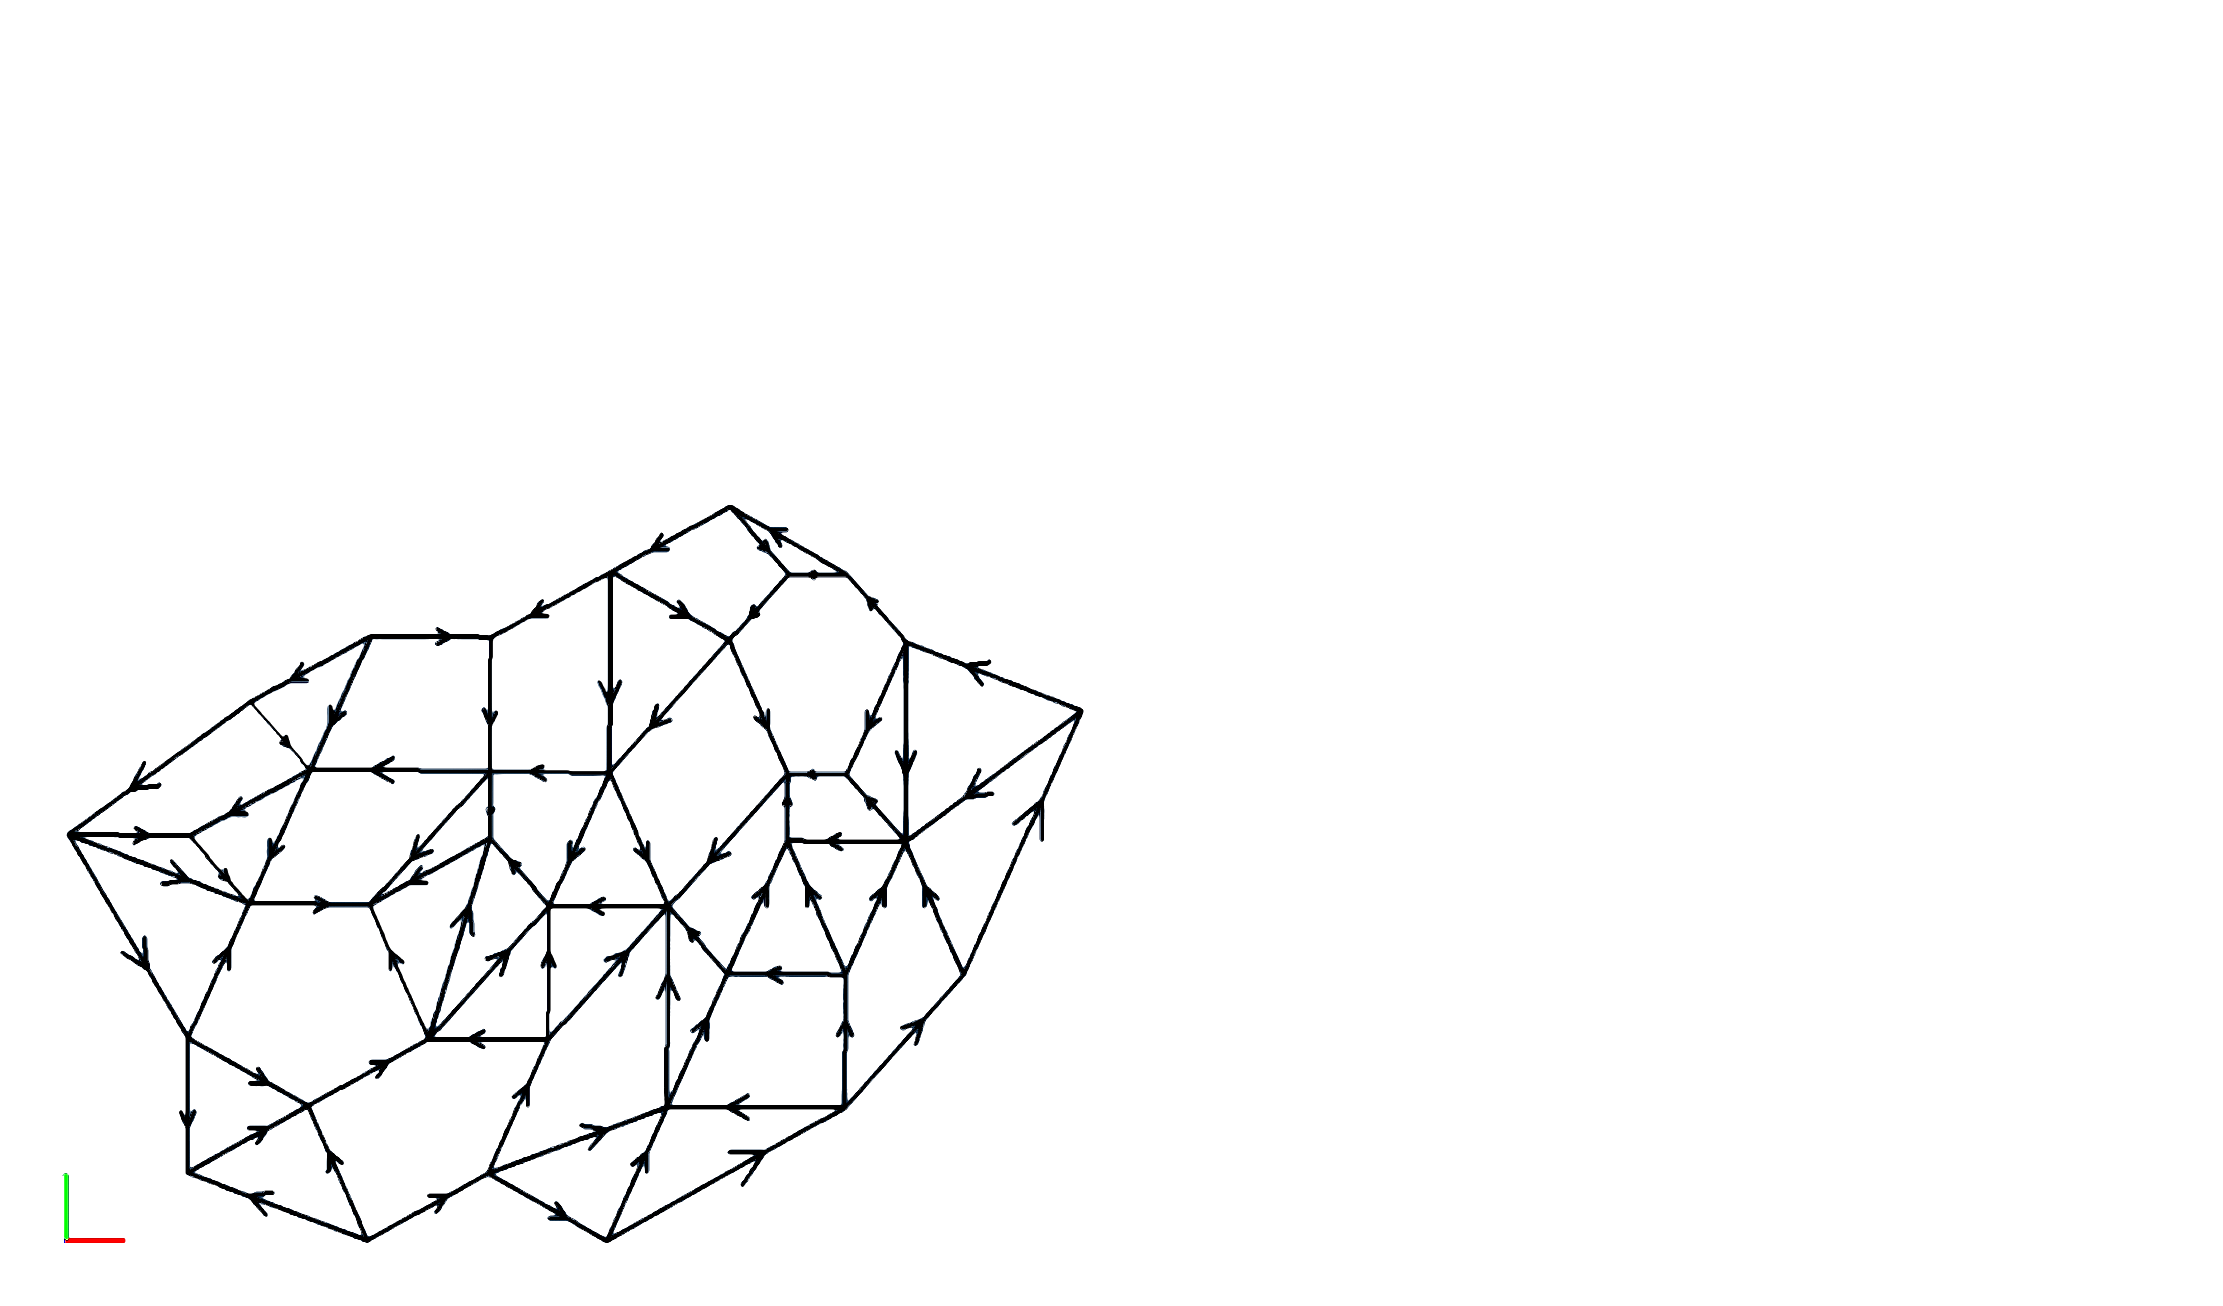
\includegraphics[width=\textwidth]{images/minimum-colors-a}
%  \caption{}
%  \vspace*{4mm}
%  \end{subfigure}
%  ~
%  \begin{subfigure}[b]{0.48\linewidth}
%  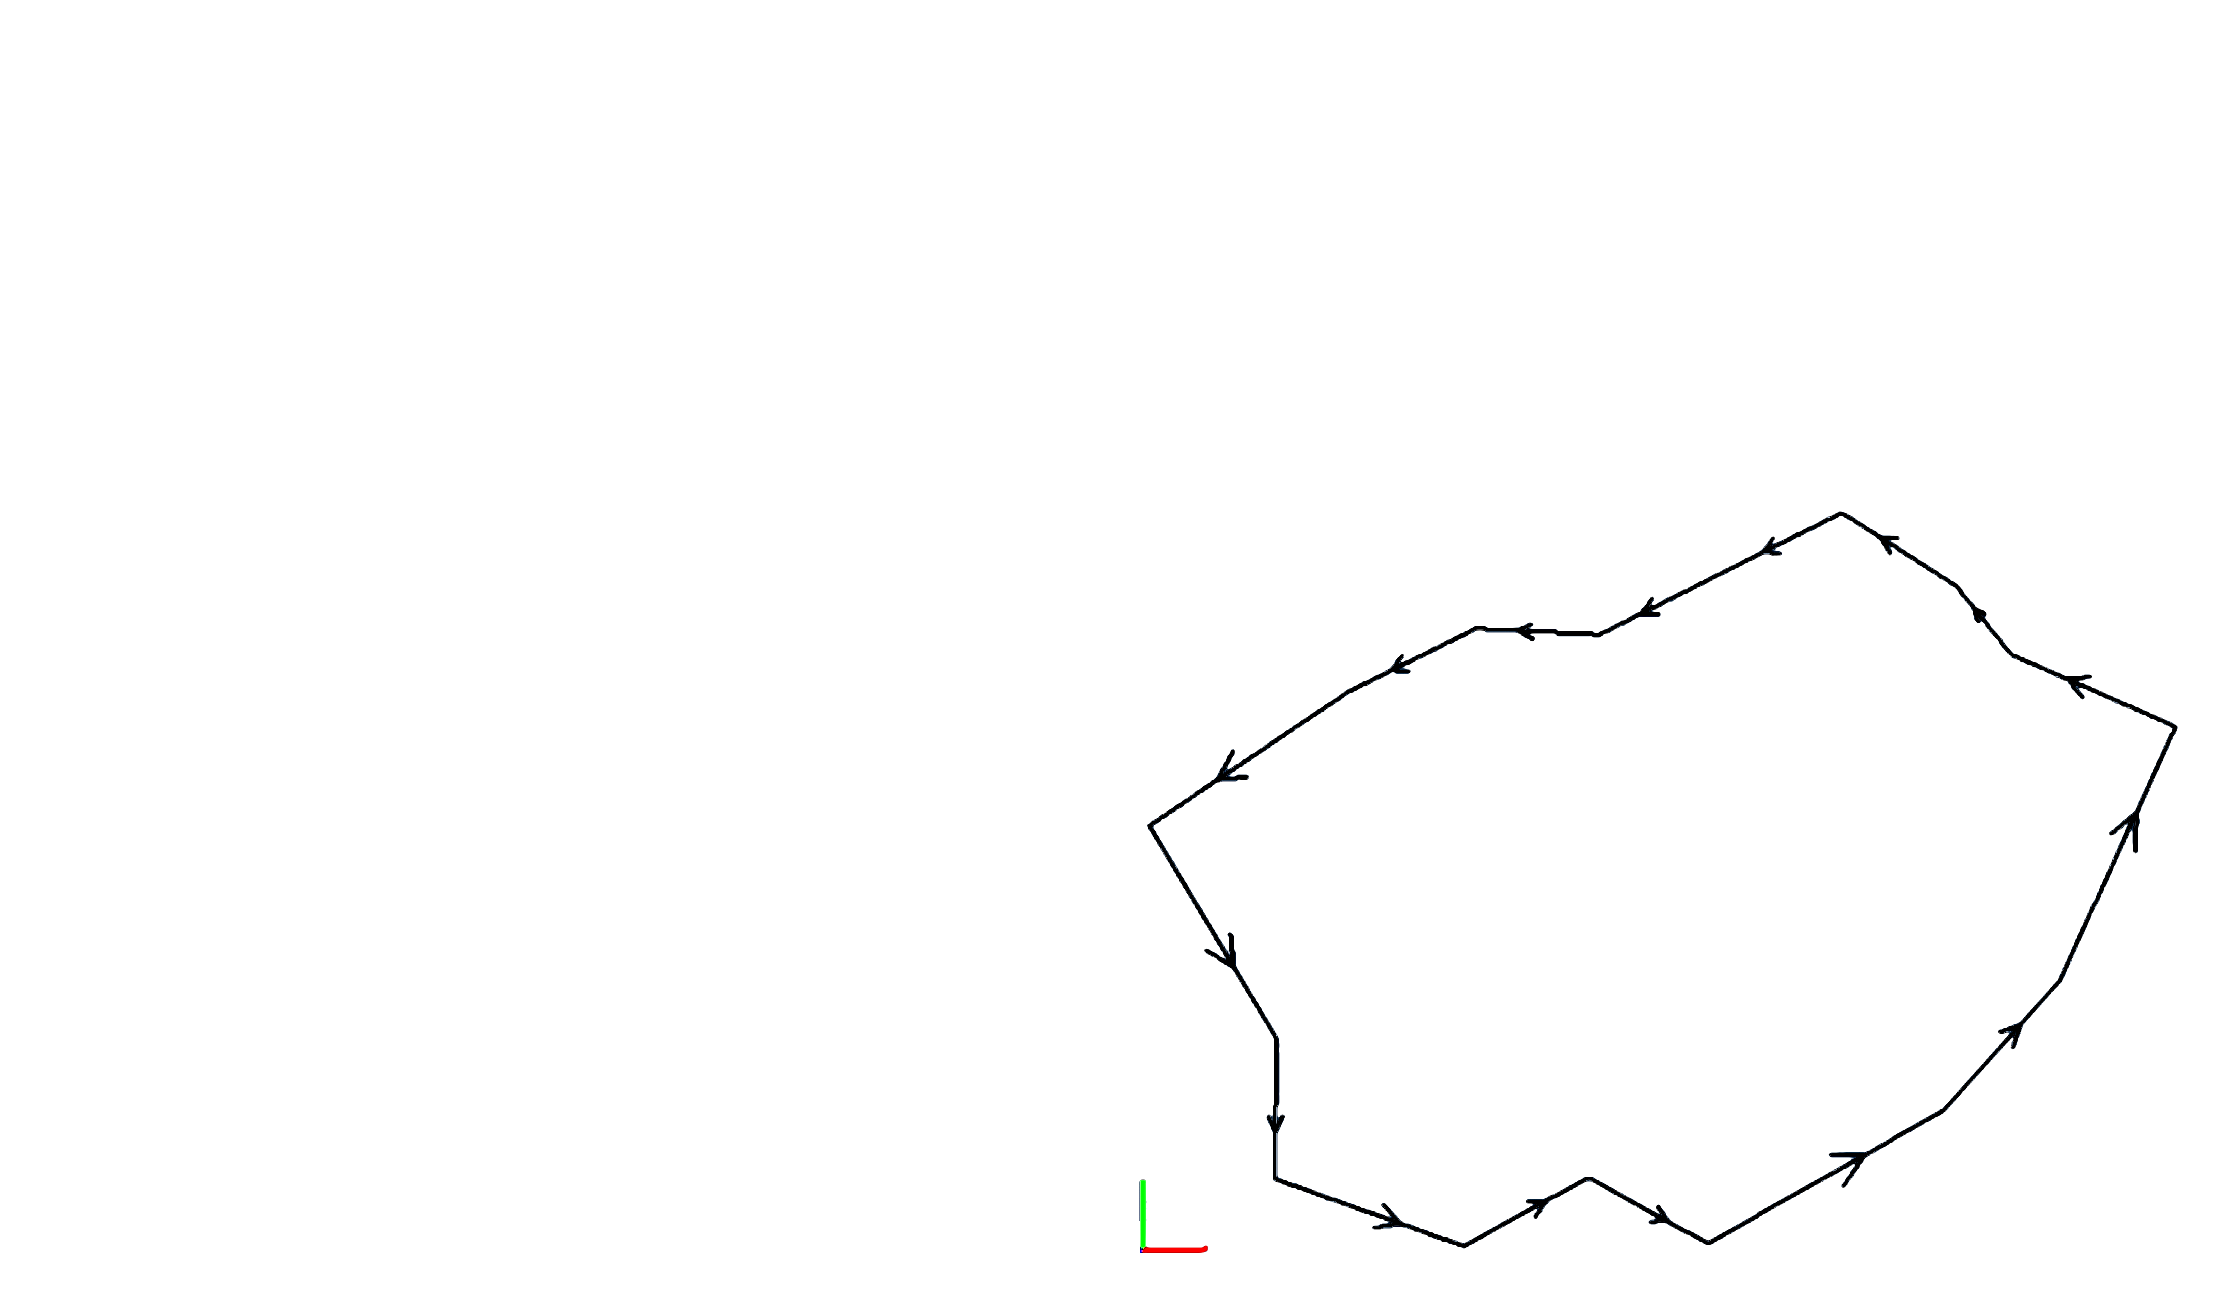
\includegraphics[width=\textwidth]{images/minimum-colors-b}
%  \caption{}
%  \vspace*{4mm}
%  \end{subfigure}
% \\
%  \begin{subfigure}[b]{0.74\linewidth}
%  \centering
%  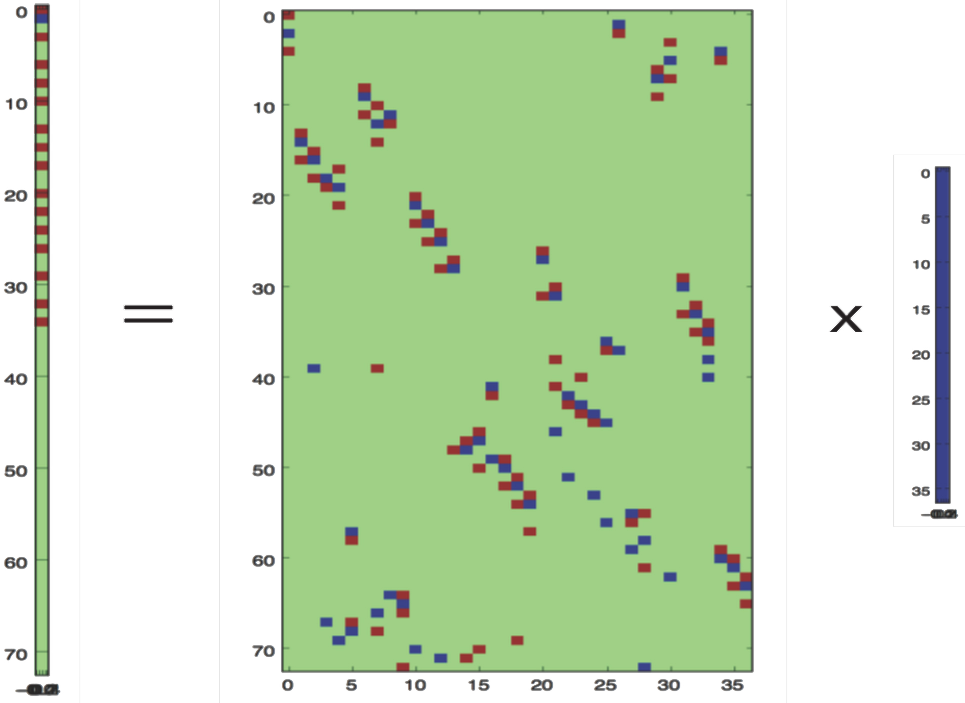
\includegraphics[width=\textwidth]{images/boundary}
%  \caption{}
%  \end{subfigure}
 
%  \caption{A toy example of the LAR scheme: (a) the bare minimum of data with \emph{complete} information about topology; (b) the extracted boundary; (c) the extraction method $[e] = [\partial][f]$ giving the coordinate representation (in the discrete basis of the 1-cells) ofthe boundary edges $[e]$ by product of the sparse boundary operator matrix $[\partial]$ times the coordinate representation $[f]$ of the 2-cells (faces), in the discrete basis of the 2-cells.}
%  \label{fig:minimum-data}
% \end{figure}

% -----------------------------------------------------------------------------


% VASTI AMBIENTI 
% MOLTI SENSORI E SISTEMI DI RILEVAZIONE DELLA POSIZIONE DIFFERENTI
% CONTINUOUS OUTDOOR-INDOOR NAVIGATION
% MONITORAGGIO DI SCENARI UNIFICATI DI INTERVENTO UOMO-MACCHINA
% PERSONALE TECNICO DEVE ESSERE GUIDATO 
% IL PASSAGGIO DA SERVER A IOT È IMMEDIATO
% MONITORAGGIO UNIFICATO DEGLI SMART OBJECTS IOT
% un ambiente indoor virtuale è l'ambiente perfetto per andare a monitorare l'IoT.

% IN QUESTO SCENARIO SI PONE IL LAVORO DESCRITTO IN QUESTO PAPER, 
% IN CUI LE NECESSIT`A DESCRITTE VENGONO AFFRONTATE PARTENDO DALLE BASI,
% OVVERO DEFINENDO UN FORMATO DI DOCUMENTO PER LA DESCRIZIONE ASTRATTA DI AMBIENTI INDOOR.
% DESCRITTO L'AMBIENTE DEVE QUINDI ESSERE POSSIBILE RICOSTRUIRE VIRTUALMENTE L'AMBIENTE
% RENDERLO LARGAMENTE ACCESSIBILE VIA WEB, E MONTARE SU QUESTA RAPPRESENTAZIONE VIRTUALE 
% LA POSSIBILIT`A DI INTERAGIRE CON GLI OGGETTI ALL'INTERNO DELL'AMBIENTE. L'INTERAZIONE DEVE CONSISTERE DA UN LATO NALLA POSSIBILIT`A DI RICEVERE INFORMAZIONI DALL'OGGETTO, MA ANCHE DI INVIARE COMANDI ALL'OGGETTP.

% SI REALIZZA IN QUESTO MODO UNO SCENARIO IN CUI UN SUPERVISORE INTERAGISCE CON L'AMBIENTE IN CUI SI MUOVE UN EXPLORER (O MANUTENTORE) POTENDO IL SUPERVISORE AVERE IMMEDIATA NOTIFICA DELLA POSIZIONE DEL MANUTENTORE, E AVENDO UN QUADRO COMPLETO FORNITO DAGLI OGGETTI SMART PRESENTI NELL'AMBIENTE REALE ASSIEME ALL'EXPLORER.

% D'ALTRA PARTE PER GRANDI SPAZI ANCHE L'EXPLORER PUO ESSERE SUPPORTATO DAL SISTEMA CHE AVENDO COMPLETA CONOSCENZA DELLA TOPOLOGIA E DELLA GEOMETRIA DELL'AMBIENTE, NONCHE DEGLI OGGETTI IN ESSO CONTENUTI, POSSIEDE TUTTE LE INFORMAZIONI NECESSARIE PER GUIDARE L'EXPLORER ATTRAVERSO L'AMBIENTE.

% NULLA IMPEDISCE DI MIXARE LE NECESSITÀ DI EXPLORER E SUPERVISOR, REALIZZANDO UN EXPLORER CHE NAVIGA NELL'AMBIENTE REALE ED IN ESSO RICEVE INFORMAZIONE E A CONTEMPO PUÒ INVIARE COMANDI AGLI SMART OBJECT INTORNO A SE.
